\section{Four NP-Complete PMU Placement Problems}
\label{sec:problem-analysis}


In this section we define four PMU placement problems (\fulls, \maxincs, \xvals, and \xvalparts) and prove their NP-Completeness. 
\xval and \xvalpart both consider measurement error detection, while
\full and \maxinc do not.  In effort to keep this proposal document relatively short, we omit the actual NP-Completeness proofs and instead present proof sketches; details can 
be found in \cite{Gyllstrom12}.
We begin this section with a high-level description of the proof strategy we
use to prove each problem is NP-Complete (Section \ref{subsec:proofstrat}).  In Section \ref{subsec:pmu-prob-stmt}, we state our four PMU placement problems and outline our NP-Completeness proofs for each.

%In this section we first define four PMU placement problems and then provide a high-level description of the proof strategy we use to prove each problem is NP-Complete.
%\yyn{In all four problems defined in this paper, we are only concerned with computing the voltage phasors of each bus (i.e., observing the buses). 
%Using the values of the voltage phasors, Ohm's Law can be easily applied to compute the current phasors of each transmission line.}
%Also, we consider networks with both injection and zero-injection buses.

\subsection{Overview of NPC Proof Strategy}
\label{subsec:proofstrat}
In this section, we outline the proof strategy we use in each of our NP-Completeness proofs. 
%In effort to keep this proposal document relatively short, we omit the actual NPC proofs and instead present proof sketches.
Our proofs follow a similar structure to those proposed by Brueni and Heath \cite{Brueni05}. The authors prove NP-Completeness by reduction from planar 3-SAT (\sats).
A 3-SAT formula, $\phi$, is a boolean formula in conjunctive normal form (CNF) such 
that each clause contains at most $3$ literals. For any 3-SAT formula $\phi$ with the sets of variables $\{v_1,v_2, \dots , v_r\}$ and clauses $\{c_1,c_2, \dots , c_s \}$, $G(\phi)$ 
is the bipartite graph $G(\phi)=(V(\phi),E(\phi))$ defined as follows:
\begin{eqnarray*}
 V(\phi) &= &\{v_i\; \vert\; 1 \leq i \leq r \} \cup \{c_j \;\vert\; 1 \leq j \leq s \} \\
 E(\phi) &=& \{ (v_i,c_j)\;\vert\; v_i \in c_j\;\; or \;\; \overline{v_i} \in c_j\}.
\end{eqnarray*}
Note that edges pass only between $v_i$ and $c_j$ nodes, and so the graph is bipartite.  \sat is a 3-SAT formula such that $G(\phi)$ is planar \cite{Lich82}. 
For example, \sat formula
\begin{eqnarray}
\varphi  &=& (\overline{v_1} \vee v_2 \vee v_3) \wedge (\overline{v_1} \vee \overline{v_4} \vee v_5) \wedge (\overline{v_2} \vee \overline{v_3} \vee \overline{v_5}) \nonumber\\
		 & & \wedge (v_3 \vee \overline{v_4}) \wedge  (\overline{v_3} \vee v_4 \vee \overline{v_5})
\label{eqn:varphi}
\end{eqnarray}
has graph $G(\varphi)$ shown in Figure \ref{fig:gvarphi}. 
Discovering a satisfying assignment for  \sat is an NPC problem, and so it can be used in a reduction to prove the complexity of the problems we address here. 

Following the approach in \cite{Brueni05}, for \sat formula, $\phi$, we replace each variable node and each clause node in $G(\phi)$ with a specially constructed set of nodes,
termed a {\em gadget}. In this work, all variable gadgets will have the same structure, and all clause gadgets have the same structure (that is different from the variable gadget structure), 
and we denote the resulting graph as $H(\phi)$. In $H(\phi)$, each {\em variable} gadget has a subset of nodes that semantically represent assigning ``True" to that variable, and a subset of 
nodes that represent assigning it ``False". When a PMU is placed at one of these nodes, this is interpreted as assigning a truth value to the \sat variable corresponding with that gadget. 
Thus, we use the PMU placement to determine a consistent truth value for each \sat variable. Also, clause gadgets are connected to variable gadgets at either ``True" or ``False" (but never both) 
nodes, in such a way that the clause is satisfied if and only if {\em at least one} of those nodes has a PMU.

While we assume $G(\phi)$ is planar, we make no such claim regarding $H(\phi)$, though in practice all graphs used in our proofs are indeed planar. The proof of NPC rests on the fact that solving the underlying $\phi$ formula is NPC.

In what follows, for a given PMU placement problem $\Pi$, we prove $\Pi$ is NPC by showing that a PMU placement in $H(\phi)$, $\Phi$, can be interpreted semantically as describing a satisfying assignment for $\phi$ iff $\Phi\in\Pi$. 
Since \sat is NPC, this proves $\Pi$ is  NPC as well. 


While the structure of our proofs is adapted from \cite{Brueni05}, the variable and clause gadgets we use to correspond to the \sat formula are novel, thus leading to a 
different set of proofs. Our work here demonstrates how the work in \cite{Brueni05} can be extended, using new variable and clause gadgets, to address a wide array of PMU placement problems.

\begin{figure}[t]

\subfigure[$G(\varphi)$ formed from $\varphi$ in Equation (\ref{eqn:varphi}).]{\label{fig:gvarphi}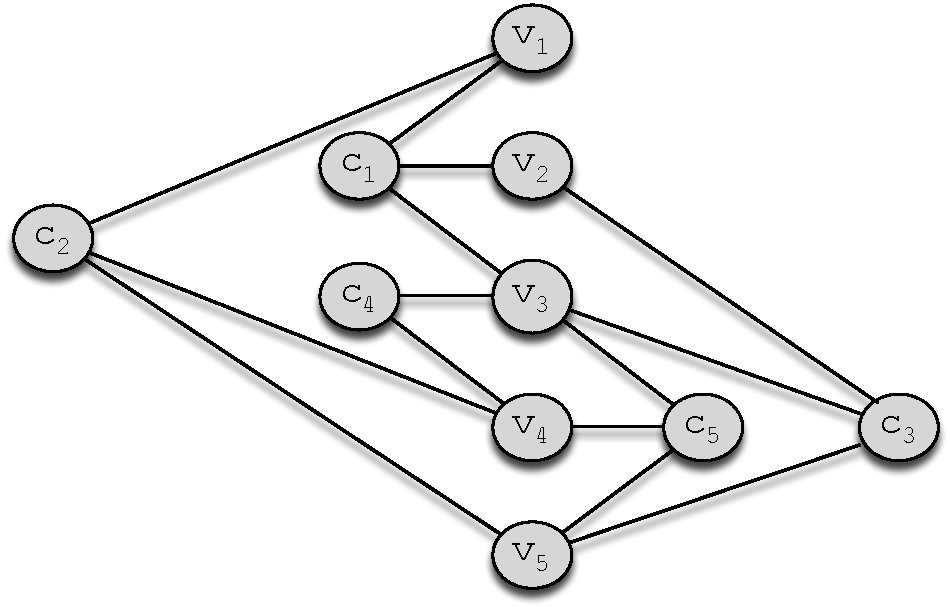
\includegraphics[scale=0.53]{figs/gvarphi.pdf}}
\subfigure[Graph formed from $\varphi$ formula in Theorem \ref{thm:npc-full} proof.] %Nodes with a dashed border are zero-injection nodes.]
{\label{fig:gvarphi2}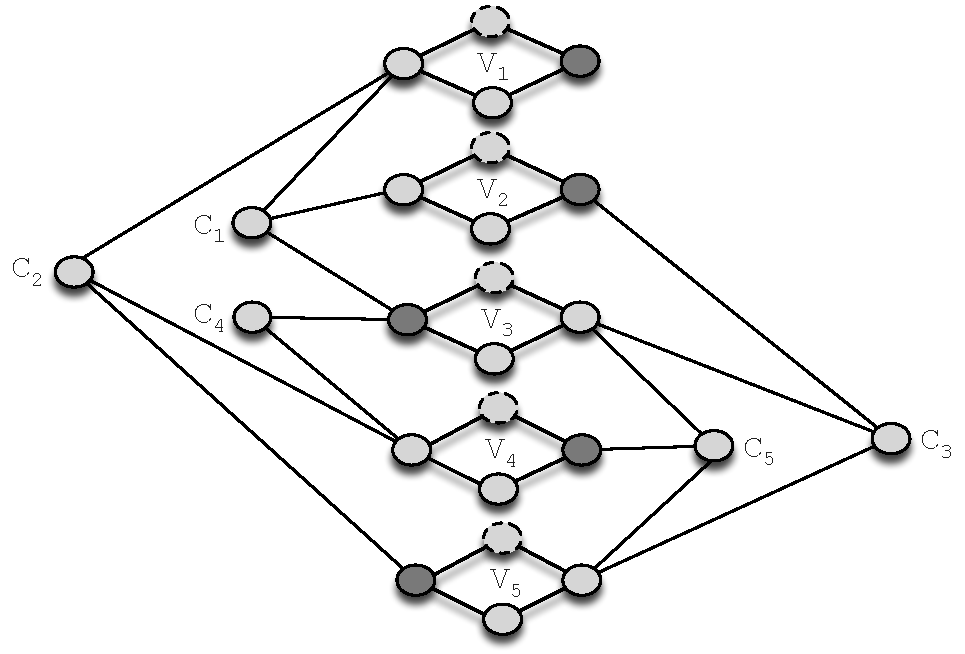
\includegraphics[scale=0.53]{figs/proof1-inject-example.pdf}}

\caption{The figure in (a) shows $G(\varphi)=(V(\varphi),E(\varphi))$ using example formula, $\varphi$, from Equation (\ref{eqn:varphi}).  (b) shows the new graph formed by replacing each variable
node in $G(\varphi)$ -- as specified by the Theorem \ref{thm:npc-full} proof -- with the Figure \ref{fig:diamond-gadget} variable gadget. 
%using the variable clause in Figure \ref{fig:diamond-gadget} and a single clause node.
} 
\end{figure}




\begin{figure}[t]
    \fbox{\subfigure[Variable gadget used in Theorem \ref{thm:npc-full} and \ref{thm:npc-maxinc}.]
	{\label{fig:diamond-gadget}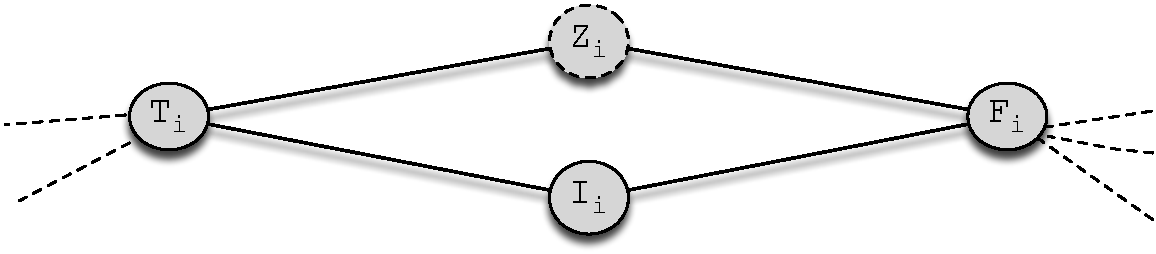
\includegraphics[scale=0.31]{figs/diamond-gadget.pdf}}}
	\fbox{\subfigure[Theorem \ref{thm:npc-maxinc} clause gadget.]
	{\label{fig:line-gadget}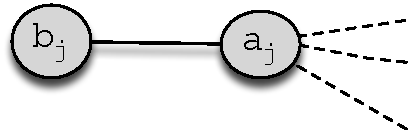
\includegraphics[scale=0.31]{figs/line-gadget.pdf}}}
	\fbox{\subfigure[Variable gadget used in Theorem \ref{thm:npc-xval}, containing two disconnected subgraphs.]
	{\label{fig:xval-gadget}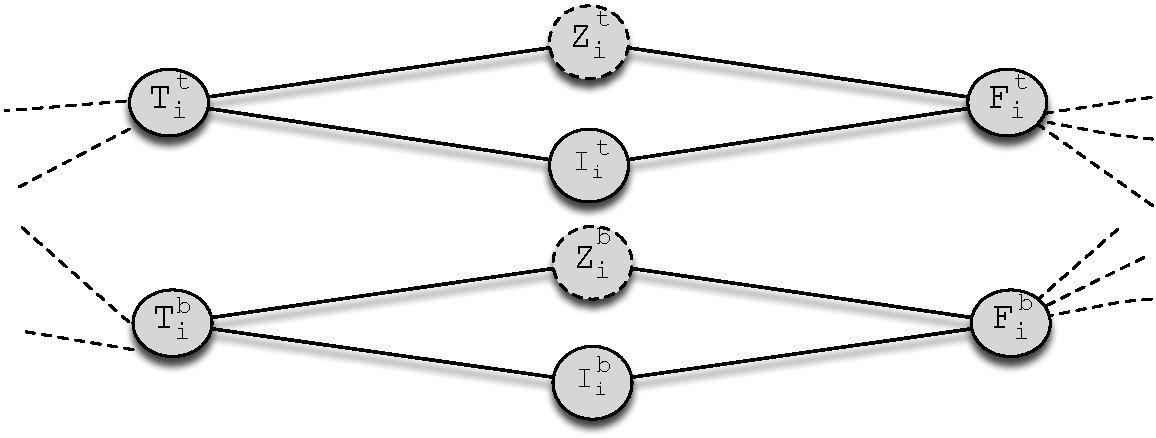
\includegraphics[scale=0.31]{figs/vgadget-inject.pdf}}}

	\caption{Gadgets used in Theorem \ref{thm:npc-full} - \ref{thm:npc-xvalpart}. $Z_i$ in Figure \ref{fig:diamond-gadget}, $Z_i^t$ in Figure \ref{fig:xval-gadget}, and $Z_i^b$ in Figure \ref{fig:xval-gadget} are the only zero-injection nodes.
	The dashed edges in Figure \ref{fig:diamond-gadget} and Figure \ref{fig:xval-gadget} are connections to clause gadgets. Likewise, the dashed edges in Figure (b) are connections to variable gadgets.  In Figure \ref{fig:xval-gadget},
	superscript, $t$, denotes nodes in the upper subgraph and superscript, $b$, indexes nodes in the lower subgraph.}
	%\caption{Graph $G=(V,E)=H_1(\varphi)$ formed from $\varphi$ formula in Theorem \ref{thm:npc-full} proof. Nodes with a dashed border are zero-injection nodes.}
  
\label{fig:pmu-gadgets}
\end{figure}

%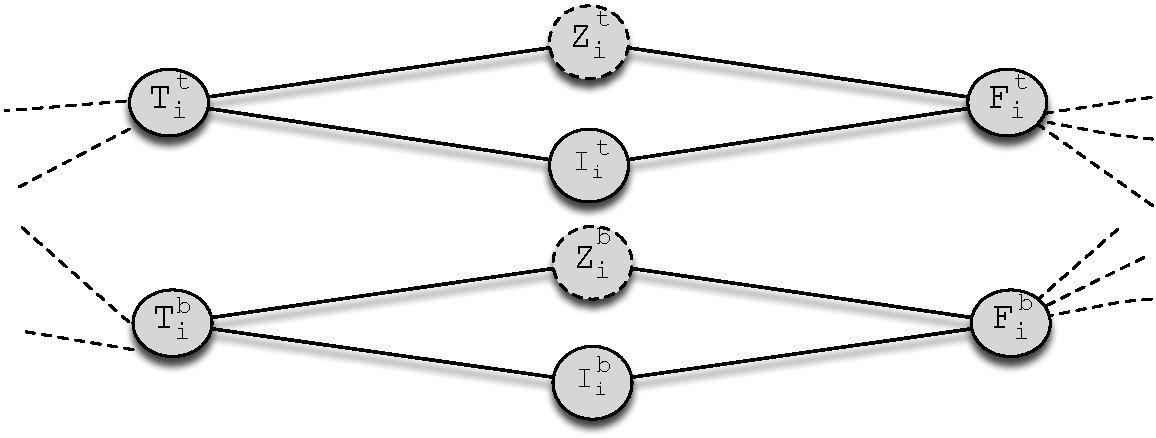
\includegraphics[scale=0.46]{figs/vgadget-inject.pdf}
%\caption{Variable gadget used in Theorem \ref{thm:npc-xval}, containing two disconnected subgraphs. Superscript, $t$, denotes nodes in the upper subgraph and 
%superscript, $b$, indexes nodes in the lower subgraph. The dashed edges are connections to clause gadgets.}
%\label{fig:xval-gadget}

%\begin{figure}[t]
%\centering
%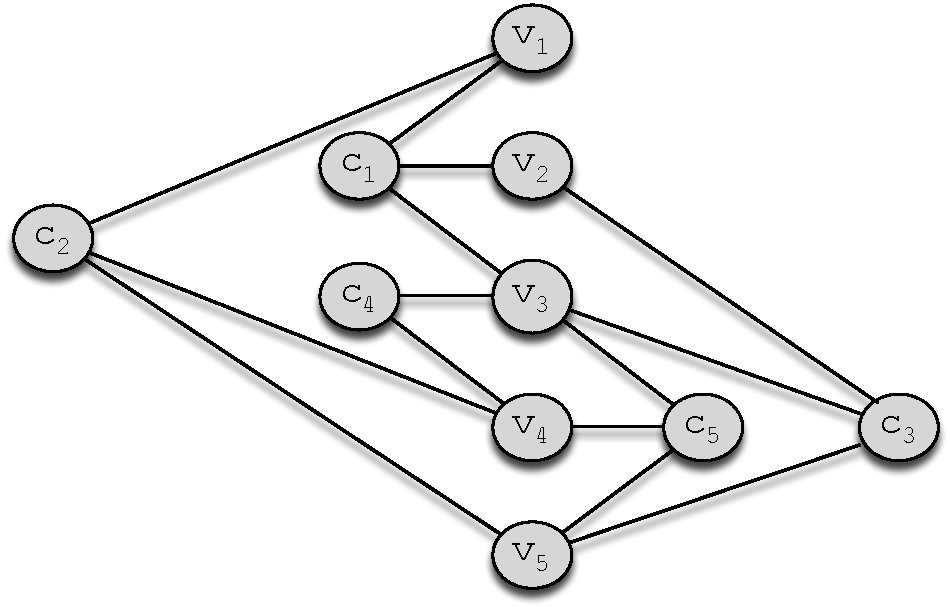
\includegraphics[scale=0.53]{figs/gvarphi.pdf}
%\caption{$G(\varphi)=(V(\varphi),E(\varphi))$ formed from $\varphi$ in Equation (\ref{eqn:varphi}). }
%\label{fig:gvarphi}
%\end{figure}


\subsection{Problem Statements and NPC Proof Sketches}
\label{subsec:pmu-prob-stmt}

Here we briefly define each of our four PMU placement problems: \fulls, \maxincs, \xvalparts, and \xvals.   Then, we provide proof sketches (that follow the proof strategy outlined in the previous section)
demonstrating that each algorithm is NP-Complete. \\ 
{\bf \full Decision Problem:} \\
\indent \underline{Instance}: Graph $G=(V,E)$ where $V=V_Z \cup V_I$, $V_Z \neq \emptyset$, $k$ PMUs such that $k \geq 1$. \\
\indent \underline{Question}: Is there a $\Phi_G$ such that $|\Phi_G| \leq k$ and $\Phi^R_G = V$? 

\begin{theorem}
\full is NP-Complete.
\label{thm:npc-full}
\end{theorem}

{\it Proof Sketch}:  We introduce a problem-specific variable gadget shown in Figure \ref{fig:diamond-gadget} and a single node as the clause gadget. We show that in order to observe all nodes, PMUs must be placed on variable gadgets, specifically on
nodes that semantically correspond to True and False values that satisfy the corresponding \sat formula. 

Consider the example \sat formula from Equation \ref{eqn:varphi}, $\varphi$, and its corresponding bipartite graph, $G(\varphi)$, shown in Figure \ref{fig:gvarphi}.  
Our proof procedure replaces each variable node in $G(\varphi)$ with the variable gadget shown in Figure \ref{fig:diamond-gadget}, 
yielding the graph shown in Figure \ref{fig:gvarphi2}. Nodes with a dashed border are zero-injection nodes.  $\varphi$ is satisfied when literals $\overline{v_1}, \overline{v_2}, v_3, \overline{v_4},$ and $\overline{v_5}$ are all True,
yielding a PMU placement with PMUs at each dark shaded node in Figure \ref{fig:gvarphi2}.
%The resulting graph for the example given in Figure \ref{fig:gvarphi} is shown in Figure \ref{fig:proof1-inject-example}.  
%Nodes with a dashed border are zero-injection nodes.  The corresponding formula for this graph, $\varphi$,
%is satisfied by truth assignment $A_{\varphi}$: $\overline{v_1}, \overline{v_2}, v_3, \overline{v_4},$ and $\overline{v_5}$ are True. This corresponds to the dark shaded nodes in Figure \ref{fig:gvarphi2}.
\\
{\bf \maxinc Decision Problem:} \\
\indent \underline{Instance}: Graph $G=(V,E)$ where $V=V_Z \cup V_I$, $k$ PMUs such that $1 \leq k < k^*$. \\
\indent \underline{Question}: For a given $m< |V|$, is there a $\Phi_G$ such that $|\Phi_G| \leq k$ and $m \leq |\Phi^R_G| < |V|$? 

\begin{theorem}
\maxinc is NP-Complete.
\label{thm:npc-maxinc}
\end{theorem}

{\it Proof Sketch}:  First, we construct problem-specific gadgets for variables (Figure \ref{fig:diamond-gadget})  and clauses (Figure \ref{fig:line-gadget}). We then demonstrate that any solution that observes $m$ nodes must place the PMUs only on nodes
in the variable gadgets. Next we show that as a result of this, the problem of observing $m$ nodes in this graph reduces to Theorem \ref{thm:npc-full}. 
\\
{\bf \xval Decision Problem:} \\
\indent \underline{Instance}: Graph $G=(V,E)$ where $V=V_Z \cup V_I$, $k$ PMUs such that $k \geq 1$. \\
\indent \underline{Question}: Is there a $\Phi_G$ such that $|\Phi_G| \leq k$ and $\Phi^R_G = V$ under the condition that each $v \in \Phi_G$ is cross-validated?

\begin{theorem}
\xval is NP-Complete.
\label{thm:npc-xval}
\end{theorem}

{\it Proof Sketch}:   We show \xval is NP-hard by reducing from \sats.  
We create a single-node gadget for clauses (as we did with \fulls) and the gadget shown in Figure \ref{fig:xval-gadget} for each variable. Each variable gadget here comprises of two disconnected components, 
and there are two $T_i$ and two $F_i$ nodes, one in each component. First, we show that each variable gadget must have $2$ PMUs for the entire graph to be observed, one PMU for each subgraph.
Then, we show that cross-validation constraints force PMUs to be placed on both $T$ nodes or both $F$ nodes.  Finally, we use the PMU placement to derive a satisfying \sat truth assignment.
\\
{\bf \xvalpart Decision Problem:} \\
\indent \underline{Instance}: Graph $G=(V,E)$ where $V=V_Z \cup V_I$, $k$ PMUs such that $1 \leq k < k^*$, and some $m<|V|$. \\
\indent \underline{Question}: Is there a $\Phi_G$ such that $|\Phi_G| \leq k$ and $m \leq|\Phi^R_G| < |V|$ under the condition that each $v \in \Phi_G$ is cross-validated?

\begin{theorem}
\xvalpart is NP-Complete.
\label{thm:npc-xvalpart}
\end{theorem}

{\it Proof Sketch}:  Our proof is a combination of the NP-Completeness proofs for \maxinc and \xvals.
